 \documentclass[9pt]{beamer}
%\documentclass[compress,9pt,usenames,dvipsnames]{beamer}
% \usepackage[utf8]{inputenc}
% \includeonlyframes{current}
\input{Common}
% If you have a file called "university-logo-filename.xxx", where xxx
% is a graphic format that can be processed by latex or pdflatex,
% resp., then you can add a logo as follows:

% \pgfdeclareimage[height=1cm]{Emory}{figs/Emory.png}


\title % (optional, use only with long paper titles)
{
  Financial Mathematics \\
  \bigskip
  \small MATH 5870/6870\footnote{\textcolor{gray}{Based on Robert L. McDonald's {\it Derivatives Markets}, 3rd Ed, Pearson, 2013.}}\\
  Fall 2021
}

% \subtitle
% {Research Plan} % (optional)

\author{Le Chen\\[1em]
  {\small\textcolor{gray}{\url{lzc0090@auburn.edu}}}
}


\institute[Auburn University]
{
% \pgfuseimage{Emory}\\[3em]
% {\small Auburn University}\\[1em]
% {\small Auburn AL}\\[3em]
\textcolor{gray}{Last updated on } \\[1em]
\textcolor{gray}{\today}
 \vspace{8em}
}
% - Use the \inst command only if there are several affiliations.
% - Keep it simple, no one is interested in your street address.

\date[Auburn]{Auburn University\\ \textcolor{gray}{Auburn AL}}
% \date{}

% \subject{}



\begin{document}
\begin{frame}[noframenumbering]
  \titlepage
\end{frame}
\newcommand{\myChapter}{Chapter 1. Introduction to Derivatives}
\newcommand{\mySection}[1]{
  \section{\S\: #1}
  \begin{frame}{\myChapter}\tableofcontents\end{frame}
  \begin{frame}{\myChapter}\tableofcontents[currentsection]\end{frame}
  }
\begin{frame}
\begin{center}
\huge
\myChapter
\end{center}
\end{frame}
\def\mySecNum{1.1}
\mySection{\mySecNum~What is a derivative?}
%-------------- start slide -------------------------------%{{{ 1
\begin{frame}[fragile,t]
	\begin{mydefinition}
		A \textcolor{magenta}{derivative} is a financial instrument that has a value determined by the price of something
		else.
	\end{mydefinition}
\end{frame}
%-------------- end slide -------------------------------%}}}
%-------------- start slide -------------------------------%{{{ 1
\begin{frame}[fragile,t]
	\begin{myexample}
		An agreement where
		\begin{center}
			you pay \$1 if the price of corn is greater than \$3 \\
			and                                                  \\
			you receive \$1 if the price of corn is less that \$1
		\end{center}
		is a derivative.
	\end{myexample}

	\bigskip
	\mySeparateLine
	\bigskip

	\begin{center}
		This contract can be used to   \\
		\bigskip
		\textcolor{magenta}{speculate} on the price of corn \\
		or                             \\
		it can be used to \textcolor{cyan}{reduce risk}.
	\end{center}
	\bigskip

	Hence, it is not the contract itself, but how it is used, and who uses it, that determines whether
	or not it is risk-reducing. It all depends on context.
\end{frame}
%-------------- end slide -------------------------------%}}}

\def\mySecNum{1.2}
\mySection{\mySecNum~An overview of financial markets}
%-------------- start slide -------------------------------%{{{ 1
\begin{frame}[fragile,t]
	The trading of a financial asset involves at least four discrete steps:
	\bigskip

	\begin{enumerate}
		\item A buyer and a seller must locate one another and agree on a price
			\bigskip
		\item The trade must be \textcolor{magenta}{cleared}\\
			(the obligations of each party are specified)
			\bigskip
		\item The trade must be \textcolor{magenta}{settled} \\
			(the buyer and the seller must deliver the cash or securities necessary to satisfy their
			obligations in the required period of time)
			\bigskip
		\item Ownership records are updated.
	\end{enumerate}
	\vfill

	\begin{center}
		\begin{tikzpicture}[scale=1, transform shape]
		\tikzset{>=latex}
		\only<1->{\node[draw] (1) at (0,0) {Striking a price};}
		\only<2->{\node[circle,draw] (2) at (2.7,0) {clearing};
			\draw[->, shorten <= 0.3em, shorten >= 0.3em] (1) -- (2);}
		\only<3->{\node[circle,draw] (3) at (5,0) {settling};
			\draw[->, shorten <= 0.3em, shorten >= 0.3em] (2) -- (3);}
		\only<4->{\node[draw] (4) at (8,0) {maintaining records};
			\draw[->, shorten <= 0.3em, shorten >= 0.3em] (3) -- (4);}
		\end{tikzpicture}
	\end{center}
\end{frame}
%-------------- end slide -------------------------------%}}}
%-------------- start slide -------------------------------%{{{ 1
\begin{frame}[fragile,t]
	There are at least four different \textcolor{cyan}{measures of a market and its activity}:
	\bigskip
	\begin{enumerate}
		\item \textcolor{magenta}{Trading volume}: the number of financial claims that change hands
			daily or annually.  \bigskip
		\item \textcolor{magenta}{Market value or market cap}: the sum of the market value of the claims
			that \textcolor{cyan}{could} be traded, without regard to whether they have traded.
			\bigskip
		\item \textcolor{magenta}{Notional value}: Notional value measure the scale of a position,
			usually with reference to some underlying asset.
			\bigskip
		\item \textcolor{magenta}{Open Interest}. Open interest measures the total number of contracts
			for which counter parties have a future obligation to perform. It is an important statistic in
			derivatives market.
	\end{enumerate}
\end{frame}
%-------------- end slide -------------------------------%}}}
%-------------- start slide -------------------------------%{{{ 1
\begin{frame}[fragile,t]

\begin{center}
	Companies typically raise funds by
	\bigskip
	\bigskip

	\renewcommand{\arraystretch}{1.2}
	\begin{tabular}{|c|c|}
		\hline
		\textcolor{magenta}{stock markets} & \textcolor{cyan}{bound markets}         \\
		\hline
		Selling ownership claims           & Obtaining a bank loan or issuing a bond \\
		Securities exchanges               & Through dealers                         \\
		(NYSE, NASDAQ)                     &                                         \\
                                       & less frequent                           \\
	  \hline
	\end{tabular}
\end{center}
\end{frame}
%-------------- end slide -------------------------------%}}}
%-------------- start slide -------------------------------%{{{ 1
\begin{frame}[fragile,t]
	The introduction of derivatives in a market often coincides with \textcolor{magenta}{an increase
	in price risk} in that market. For example,
\begin{enumerate}
	\item Currencies were permitted to float in 1971 when the gold standard was officially abandoned.
		The modern market in financial derivatives began in 1972, when the \textcolor{cyan}{Chicago
		Mercantile Exchange} started trading futures contracts on seven currencies.
	\item OPEC’s 1973 reduction in the supply of oil was followed by high and variable oil prices.
	\item U.S. interest rates became more volatile following inflation and recessions in the 1970s.
	\item The market for natural gas has been deregulated gradually since 1978, resulting in a
		volatile market in recent years.
	\item The deregulation of electricity began during the 1990s.
\end{enumerate}
\end{frame}
%-------------- end slide -------------------------------%}}}
%-------------- start slide -------------------------------%{{{ 1
\begin{frame}[fragile,t]
	\begin{center}
	History of the crude oil prices  \bigskip \bigskip

	\includegraphics[scale=0.25]{figs/crude-oil-price-history-chart-neg.png}\footnote{Image from
	\url{https://www.macrotrends.net/}}
	\bigskip

	\end{center}
\end{frame}
%-------------- end slide -------------------------------%}}}
%-------------- start slide -------------------------------%{{{ 1
\begin{frame}[fragile,t]

\begin{center}
 Price variability leads to the development of derivatives markets to efficiently share risk.
 \bigskip \bigskip

 \includegraphics[scale=0.3]{figs/Figure1-1-d.png}
 \bigskip

 Millions of future contracts traded annually at the Chicago Board of Trade (CBT), Chicago
 Mercantile Exchange (CME), and the New York Mercantile Exchange (NYMEX), 1970-2011.
\end{center}
\end{frame}
%-------------- end slide -------------------------------%}}}
%-------------- start slide -------------------------------%{{{ 1
\begin{frame}[fragile,t]
\begin{center}
	Examples of underlying assets on which futures contracts are traded: \bigskip

	\includegraphics[scale=0.25]{figs/Table1-2.png}
\end{center}
\end{frame}
%-------------- end slide -------------------------------%}}}
%-------------- start slide -------------------------------%{{{ 1
\begin{frame}[fragile,t]
	\frametitle{The role of financial markets}
	\begin{center}
	Insurance companies and individual communities/families have traditionally helped each other to share risks.
	\pause
	\bigskip
	\mySeparateLine
	\bigskip

	Markets make \textcolor{alert}{RISK-SHARING} more efficient \\
	\bigskip
	\renewcommand{\arraystretch}{1.2}
	\begin{tabular}{c|c|c}
		\textcolor{magenta}{Diversifiable risks}  & vanishes                 & lightening strike  \\
		\textcolor{cyan}{Non-diversifiable risks} & are reallocated to those & Stock market crash \\
                                              & most willing to hold it  &                    \\
	\end{tabular}
	\bigskip
	\bigskip
	\pause

	The existence of risk-sharing mechanisms benefits everyone!
	\end{center}
\end{frame}
%-------------- end slide -------------------------------%}}}

\def\mySecNum{1.3}
\mySection{\mySecNum~The use of derivatives}
%-------------- start slide -------------------------------%{{{ 1
\begin{frame}[fragile,t]
	\frametitle{Common reasons to use derivatives}
	\begin{enumerate}
		\item \textcolor{magenta}{Risk management}. Derivatives are a tool for companies and other users
			to reduce risks ($\sim$ \textcolor{cyan}{hedging}). Every form of insurance is a derivative.
			\bigskip
		\item \textcolor{magenta}{Speculation}. Derivatives can serve as investment vehicles ($\sim$
			\textcolor{cyan}{betting}).
			\bigskip
		\item \textcolor{magenta}{Reduce transaction costs}. Sometimes derivatives provide a lower cost
			way to undertake a particular financial transaction.
			\bigskip
		\item \textcolor{magenta}{Regulatory arbitrage}. It is sometimes possible to circumvent
			regulatory restrictions, taxes, and accounting rules by trading derivatives.
	\end{enumerate}
\end{frame}
%-------------- end slide -------------------------------%}}}
%-------------- start slide -------------------------------%{{{ 1
\begin{frame}[fragile,t]
	\frametitle{Three perspectives on derivatives}
	\begin{center}
\renewcommand{\arraystretch}{1.2}
	\begin{tabular}{|c|c|c|}
		\textcolor{magenta}{End users} & \textcolor{magenta}{Intermediaries} & \textcolor{magenta}{Economic Observers} \\ \hline
    Corporations                   & Market-makers                       & Regulators                              \\
    Investment managers            & Traders                             & Researchers                             \\
    investors                      &                                     &                                         \\ \hline
		How to use a derivative        & Mathematical details of             & Make sense of the market                \\
    to meet the goal               & pricing and hedging                 &                                         \\
	\end{tabular}

	\end{center}
\end{frame}
%-------------- end slide -------------------------------%}}}
%-------------- start slide -------------------------------%{{{ 1
\begin{frame}[fragile,t]
	\begin{center}
		New securities can be designed by using existing securities
		\bigskip

		\textcolor{magenta}{Financial engineering} is the construction of \\
		a financial product from other products.

		\pause \bigskip \mySeparateLine \bigskip

		Principles for financial engineering (or security design):

		\bigskip

		\begin{minipage}{0.7\textwidth}
		\begin{enumerate}
			\item Facilitate hedging of existing positions
			\item Allow for creation of customized products
			\item Enable understanding of complex positions
			\item Render regulation less effective
		\end{enumerate}
		\end{minipage}
	\end{center}
\end{frame}
%-------------- end slide -------------------------------%}}}


\def\mySecNum{1.4}
\mySection{\mySecNum~Buying and short-selling financial assets}
%-------------- start slide -------------------------------%{{{ 1
\begin{frame}[fragile,t]
	\frametitle{Transaction costs and the bid-ask spread}
\begin{mydefinition}
	The price at which one can buy is called the \textcolor{magenta}{offer price} or \textcolor{magenta}{ask price},
	and the price at which one can sell is called the \textcolor{magenta}{bid price}. The difference
	between the ask price and the bid price is called the \textcolor{magenta}{bid-ask spread}.
\end{mydefinition}
\bigskip
\bigskip

\begin{center}
	Terminology is in the perspective\\ of market-maker
	\bigskip

	\renewcommand{\arraystretch}{1.2}
	\begin{tabular}{|c|c|c|}
		\hline
                 & Ask (offer) price & Bid price \\ \hline
   End users     & Buy               & Sell      \\
   Market makers & Sell              & Buy       \\ \hline
	\end{tabular}
\end{center}
\end{frame}
%-------------- end slide -------------------------------%}}}
%-------------- start slide -------------------------------%{{{ 1
\begin{frame}[fragile,t]
\begin{center}
	Transaction costs \bigskip\bigskip

\renewcommand{\arraystretch}{1.2}
	\begin{tabular}{c|c}
		\textcolor{magenta}{Commission} & \textcolor{cyan}{bid-ask spread} \\ \hline
    Brokers                         & Market-makers                    \\
    Electronic trading system       &                                  \\ \hline
    Fixed amount per transaction    & Based on per share               \\
    or percentage of purchase price &                                  \\
	\end{tabular}
\end{center}
\end{frame}
%-------------- end slide -------------------------------%}}}
%-------------- start slide -------------------------------%{{{ 1
\begin{frame}[fragile,t]
	\begin{myexample}
		 Buy and sell 100 shares of XYZ with
		 \begin{center}
		 	 bid = \$49.75, \quad  offer = \$50, \quad  commission = \$15.
		 \end{center}
		 What is the transaction cost?
	\end{myexample}
	\bigskip
	\pause

	\begin{mysol}
		\begin{enumerate}
			\item Buy:
				\begin{align*}
					(100 \times \$50) + \$15 = \$5,015.
				\end{align*}
			\item Sell:
				\begin{align*}
					(100 \times \$49.75) - \$15 = \$4,960.
				\end{align*}
			\item Transaction cost:
				\begin{align*}
					 \$5,015 - \$4,960 = \$55.
				\end{align*}
		\end{enumerate}
		(Note that We have payed twice the commission.)
		\myEnd
	\end{mysol}
\end{frame}
%-------------- end slide -------------------------------%}}}
%-------------- start slide -------------------------------%{{{ 1
\begin{frame}[fragile,t]
	\frametitle{Ways to buy or sell}
	\begin{center}
	\renewcommand{\arraystretch}{1.2}
		\begin{tabular}{c|c|c|}
					 & \textcolor{magenta}{Market order} & \textcolor{cyan}{Limited order} \\ \hline
			Pros & Filled immediately                & Might not be filled             \\
			Cons & Price could be better             & At a better price               \\
		\end{tabular}
	\end{center}
	\bigskip

	\begin{enumerate}
		\item \textcolor{magenta}{Market order}: an instruction to trade a specific quantity of the asset
			immediately, at the best price that is currently available.
			\bigskip

		\item \textcolor{cyan}{Limited order}: an instruction to trade a specific quantity of the asset
			at a specified price.
			\bigskip

		\item Others such as \textcolor{red}{stop-loss order}.
	\end{enumerate}
\end{frame}
%-------------- end slide -------------------------------%}}}
%-------------- start slide -------------------------------%{{{ 1
\begin{frame}[fragile,t]
	\frametitle{Long vs short positions}
\begin{center}
	\begin{center}
		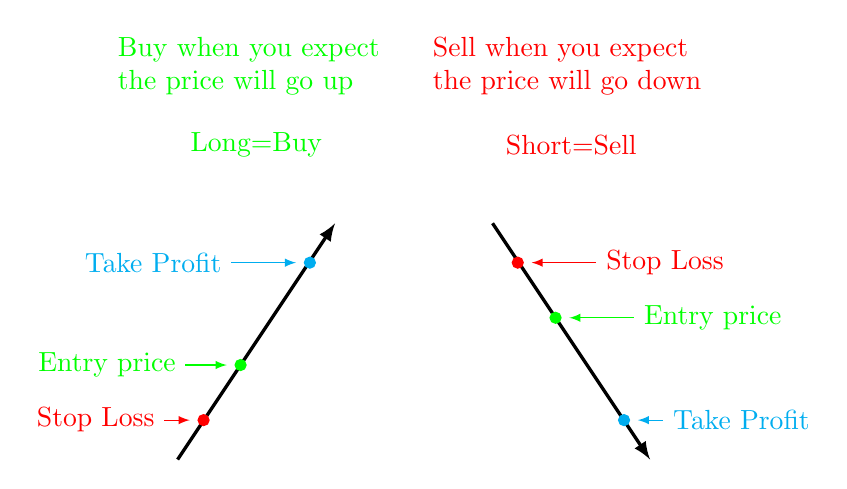
\begin{tikzpicture}[scale=1, transform shape]
			\tikzset{>=latex}
			% \node[green] (1) at (-2,3) {Lending};
			% \node[red] (1) at (2,3) {Borrowing};

			\node[green,text width=10em] (1) at (-2,2) {Buy when you expect the price will go up};
			\node[red,text width=10em] (1) at (2,2) {Sell when you expect the price will go down};
			\node[green] at (-2,1) {Long=Buy};
			\node[red] at (2,1) {Short=Sell};

			\draw[->,very thick] (-3,-3) -- (-1,0);
			\draw[->,very thick] (1,0) -- (3,-3);
			\filldraw[red] (-2.67,-2.5) circle (2pt);
			\draw [<-,red, shorten <= 0.5em] (-2.67,-2.5) -- ++ (-0.5,0) node [left] {Stop Loss};
			\filldraw[cyan] (2.67,-2.5) circle (2pt);
			\draw [<-,cyan, shorten <= 0.5em] (2.67,-2.5) -- ++ (0.5,0) node [right] {Take Profit};
			\filldraw[red] (1.32,-0.5) circle (2pt);
			\draw [<-,red, shorten <= 0.5em] (1.32,-0.5) -- ++ (1,0) node [right] {Stop Loss};
			\filldraw[cyan] (-1.32,-0.5) circle (2pt);
			\draw [<-,cyan, shorten <= 0.5em] (-1.32,-0.5) -- ++ (-1,0) node [left] {Take Profit};
			\filldraw[green] (-2.2,-1.8) circle (2pt);
			\draw [<-,green, shorten <= 0.5em] (-2.2,-1.8) -- ++ (-0.7,0) node [left] {Entry price};
			\filldraw[green] (1.8,-1.2) circle (2pt);
			\draw [<-,green, shorten <= 0.5em] (1.8,-1.2) -- ++ (1,0) node [right] {Entry price};
			% \node[bride,minimum size=1.5cm] (T) at (-1,0) {};
			% \node[groom,mirrored,minimum size=1.5cm] (N) at (1,0) {};
		\end{tikzpicture}
	\end{center}
\end{center}
\end{frame}
%-------------- end slide -------------------------------%}}}
%-------------- start slide -------------------------------%{{{ 1
\begin{frame}[fragile]
	\frametitle{Short-selling}
\begin{center}
	\begin{tikzpicture}[scale=1, transform shape]
		\tikzset{>=latex}
		\node[businessman,minimum size=3em] (T) at (-3,0) {Broker};
		\node[duck,mirrored,minimum size=3em] (N) at (0,0) {Short seller};
		\node[judge,mirrored,minimum size=3em] (N) at (3,0) {Market};
		\draw [->] (-2,0.5) -- (-1,0.5);
		\draw [->] (-1,-0.5) -- (-2,-0.5);
		\draw [->] (1,0.5) -- (2,0.5);
		\draw [->] (2,-0.5) -- (1,-0.5);
		\node[text width=8em,align=center] at (-1.5,1.4) {Borrow shares at low price};
		\node[text width=4em,align=center] at (-1.5,-1.7) {Return shares};

		\node[text width=8em,align=center] at (1.5,1.4) {Sold at current market price};
		\node[text width=8em,align=center] at (1.5,-2.2) {When market price fall, buy them at lower price};
	\end{tikzpicture}
\end{center}
\end{frame}
%-------------- end slide -------------------------------%}}}
%-------------- start slide -------------------------------%{{{ 1
\begin{frame}[fragile,t]
\begin{myexample}
	Short-sell IBM stock for 90 days. \\
	\bigskip
\begin{center}
	\renewcommand{\arraystretch}{1.2}
	\begin{tabular}{|c|c|c|c| c|}
		\hline
             & Day zero      & Dividend Ex-Day & Day $90$        & Profit          \\ \hline
   Action    & Borrow shares &                 & Return shares   &                 \\
   Security  & Shell shares  &                 & Purchase shares &                 \\
	 Cash flow & $+S_0$        & $-D$            & $-S_{90}$       & $ S_0-D-S_{90}$ \\ \hline
	\end{tabular}
\end{center}
\end{myexample}
\end{frame}
%-------------- end slide -------------------------------%}}}
%-------------- start slide -------------------------------%{{{ 1
\begin{frame}[fragile,t]
Three reasons to short-sell
\begin{enumerate}
	\item Speculation
	\item Financing
	\item Hedging
\end{enumerate}

\bigskip
\mySeparateLine
\bigskip

Credit risk in short-selling
\begin{itemize}
	\item The lender holding the money with an extra called \textcolor{magenta}{Haircut}.
\end{itemize}
\bigskip

Interest received from lender
\begin{itemize}
	\item Scarcity decreases the interest rate.
	\item \textcolor{magenta}{Repo rate} in bound markets.
	\item \textcolor{magenta}{Short rebate} in the stock market.
\end{itemize}
\end{frame}
%-------------- end slide -------------------------------%}}}

\def\mySecNum{1.5}
\mySection{\mySecNum~Problems}
%-------------- start slide -------------------------------%{{{ 1
\begin{frame}[fragile,t]
	Problems:
	1.3,
	1.4,
	1.5,
	1.6,
	1.7,
	1.11,
	1.14.
	\\
	\bigskip

	Due Date: TBA
\end{frame}
%-------------- end slide -------------------------------%}}}

\end{document}
